\chapter{Literature Review}

\section{Cloth Simulation}
The simulation of cloth is a relatively old and well studied field with applications in many different areas, including, but not limited to:
\begin{itemize}
  \item{Virtual Garment Design}
  \item{Virtual Fitting Rooms}
  \item{Films}
  \item{Video Games}
\end{itemize}
Different use cases require different things from the cloth simulation. For example, in virtual garment design, the physical accuracy of the simulation is paramount whereas cloth simulation for video games prioritises real-time simulation, sacrificing accuracy. Hence, many different models for cloth simulation have been proposed.
\\Since this project is concerned with the real-time simulation of cloth, only those models appropriate for real-time simulations have been studied in detail. However, a brief overview of other techniques will be provided. For a more detailed overview of cloth simulation techniques, see \textcite{Ng1996}.

\subsection{Cloth Properties}
Cloth has several properties that should be considered for modelling.

\subsubsection{Mechanical Properties}
Cloth has three mechanical properties that control its behaviour; stretching, shearing and bending, fig. \ref{fig:mechanical properties} shows how each property affects the cloth.
\\Stretching is the displacement of the cloth in either the horizontal or vertical direction. Most cloth has a high resistance to stretching and can typically only be stretched by 10\% \parencites[1]{Yalcn}[4]{Provot2001}.
\\Shearing is the displacement of the cloth in a diagonal direction. Again, most cloths have high shearing resistance and this, coupled with high stretch resistance, makes cloth incompressible.
\\Finally, bending is the overall curvature of the cloth surface. Typically, cloth has low bending resistance and so is easily folded.
\begin{figure}[tp]
   \begin{center}
     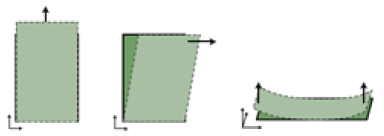
\includegraphics{Figures/mechanical_properties}
   \end{center}
   \caption[Mechanical properties of cloth]{Mechanical properties of cloth \parencite[1]{Yalcn}}
   \label{fig:mechanical properties}
\end{figure}

\subsubsection{Visual Properties}
\label{sec:visual properties}
The mechanical properties of cloth, discussed above, cause cloth to exhibit two visual properties. These properties arise from the fact that cloth is typically non-elastic, due to stretch and shear resistances, but highly flexible, due to low bend resistance.
\\Firstly, cloth will drape over objects and secondly the cloth will form many folds and wrinkles. Fig \ref{fig:visual properties} demonstrates the visual properties of cloth.
\begin{figure}[tp]
   \begin{center}
     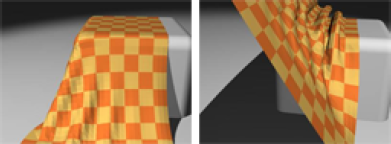
\includegraphics{Figures/visual_properties}
   \end{center}
   \caption[Visual Properties of cloth]{Visual properties of cloth \parencite[1]{Yalcn}}
   \label{fig:visual properties}
\end{figure}

\subsection{Cloth Models}
Techniques for modelling cloth are usually classified as either Geometric or Physically-based, and the choice of which modelling method to use depends on the use-case for the simulation.

\subsubsection{Geometric Models}
This family of techniques were the first models used to simulate cloth. They model the cloth using geometric equations and are especially good at modelling folds and wrinkles.
\\Weil was the first to propose a geometric model in 1986 and uses catenary curves to model the drape and folds of a hanging cloth. Following on from Weil, a number of other geometric models were proposed (see \textcite{Ng1996} for more information).
\\All geometric techniques focus on simulating the appearance of cloth, rather than the physical properties. As such, geometric models are typically more computationally efficient than physically-based models, as there is no need to solve a series of complex equations. However, geometric techniques are unable to accurately simulate the motion of cloth, \parencites[1]{Mongus2012}[2]{Zhang2001}[1-2]{Xinrong2009}, and so are mostly useful for static cloth simulations.
\\As such, geometric models have not been considered for this project.

\subsubsection{Physically-based Models}
By contrast, physically-based models are concerned with the accurate modelling of the physical properties of the cloth and can therefore be used to produce realistic animations.
\\These models typically use a system of partial differential equations (PDE), or other differential equations, to model the cloth. These equations cannot be solved analytically and therefore the system requires discretisation to solve the equations at specific points in space and time. Following discretisation, a physically-based model typically requires the solving of an ordinary differential equation (ODE) of the form \parencite[1]{Baraff1998}:
\begin{equation}
\begin{split}
\label{eq:general ODE}
  &\ddot{x} = M^{-1}\bigg(-\frac{\delta E}{\delta x} + F\bigg)
  \\\text{where:}
  \\&\text{x is a vector representing the geometric state of the system}
  \\&\text{M is a diagonal matrix representing the mass distribution of the system}
  \\&\text{E is a function of x which yields the internal cloth energy}
  \\&\text{F is a function of x and }\dot{x}\text{ which describes other forces}
  \end{split}
\end{equation}
\\Physically-based models can be classified as either Continuum or Discrete.

\paragraph{Continuum Models}\leavevmode\\
Continuum models were the first physical models to be proposed. Techniques in this family model cloth as a continuous surface and utilise continuum mechanics to calculate its behaviour; the Lagrange equations are most commonly used.
\\To discretise the continuous model, a numerical technique, such as a finite element method, is used. This is one of the advantages of continuum methods; they allow the use of a low resolution discretisation without sacrificing the accuracy of the simulation \parencite[4-5]{Wacker2005a}.
\\Another advantage of continuum models are that they are accurate; "they provide accurate models of the material derived directly from mechanical laws and models of material properties" \parencite[200]{Magnenat-Thalmann2006}.
\\This accuracy comes at the cost of computational performance, the main disadvantage of these techniques. The accuracy also renders these models inappropriate for use in dynamic simulations; "the formal and analytical description they require for the mechanical behavior of the material cannot easily be altered to represent transitory and non-linear events. Hence, phenomena such as frequent collisions or other highly variable geometrical constraints cannot be conveniently taken into account" \parencite[200]{Magnenat-Thalmann2006}. 
\\Hence, continuum models are typically only considered appropriate for static simulations, or simulations where accuracy is paramount. As a result, continuum models have not been considered.

\paragraph{Discrete Models}\leavevmode\\
According to \textcite[2]{Choi2002}, "Cloth is not a homogeneous continuum. Therefore modeling fabrics as a continuum and employing FEM or FDM has several potential drawbacks". As a result several discrete, or particle, models have been proposed.
\\With these techniques the discretisation in space is carried out by modelling the cloth as a discrete mesh, either regular or triangular, of point masses, called particles. This sacrifices some of the accuracy of continuum models, as the accuracy will depend on the number of particles used. However, this loss in accuracy is traded off against better computational performance; physical models are the only models that can be used for dynamic, real-time simulations. The discretisation of the cloth has a direct affect on the performance of the simulation; \textcite[5]{Volino2001} have shown that simulation time varies cubically with mesh size. Hence, there is a trade off to be made between accuracy and performance when using physically-based models, depending on the use-case.
\\By far the most popular technique is the mass-spring model. This model is popular as it is simple, easy to implement and offers a good balance between accuracy and efficiency. This model is the most common model used for dynamic, real-time simulations and as such, it has been chosen for this project and will now be described in more detail.

\subsection{Mass-Spring Models}
Mass-spring models were first proposed for use in cloth simulation in \textcite{Provot2001}. Using these models, the cloth is discretised as a 2-dimensional mesh of point masses, either regular or triangular, connected by linear springs.

\subsubsection{Provot Model}
Using the mass-spring model proposed in \textcite{Provot2001} the cloth is modelled as a regular mesh of point masses. The points are connected together using three different types of springs:
\begin{itemize}
  \item{Structural springs, connecting particle [i, j] to particles [i + 1, j] and [i, j + 1]. These springs resist structural deformations of the cloth, and provide the overall cloth structure. Structural springs are not enough to provide a realistic cloth model. Fig \ref{fig:structural only} shows the results of running a cloth simulation with structural springs only. As can be seen, this does not produce a realistic image}
  \item{Shear springs, connecting particle [i, j] to particle [i + 1, j + 1] and particle [i + 1, j] to particle [i, j + 1]. These springs provide shearing resistance for the cloth. By adding shear springs, the realism of the model is improved; Fig \ref{fig:structural and shear} shows the improved fidelity afforded by shear springs}
  \item{Bend springs, connecting particle [i, j] to particles [i + 2, j] and [i, j + 2]. These springs model bend resistance}
\end{itemize}

\begin{figure}
\centering
\subfigure[Initial configuration]{\label{fig:structural initial}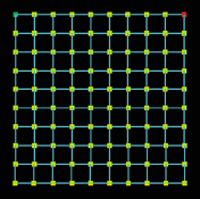
\includegraphics[width=60mm]{Figures/lander_02.png}}
\subfigure[Result of running the simulation]{\label{fig:structural results}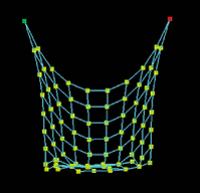
\includegraphics[width=60mm]{Figures/lander_03.png}}
\caption[Cloth with structural springs only]{Cloth with structural springs only \parencite[2]{Lander2000}}
\label{fig:structural only}
\end{figure}

\begin{figure}
\centering
\subfigure[Initial configuration]{\label{fig:shear initial}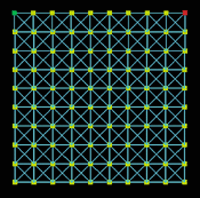
\includegraphics[width=60mm]{Figures/lander_04.png}}
\subfigure[Result of running the simulation]{\label{fig:shear results}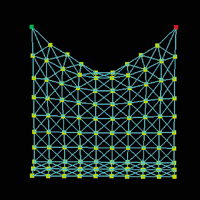
\includegraphics[width=60mm]{Figures/lander_05.png}}
\caption[Cloth with structural and shear springs]{Cloth with structural and shear springs \parencite[2]{Lander2000}}
\label{fig:structural and shear}
\end{figure}

Fig \ref{fig:provot model} shows the arrangement of these springs for a small cloth model.
\begin{figure}[tp]
   \begin{center}
     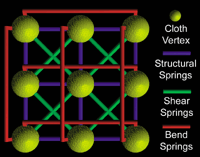
\includegraphics{Figures/provot_mesh_structure.png}
   \end{center}
   \caption[Provot cloth model]{Provot cloth model \parencite[2]{Lander2000}}
   \label{fig:provot model}
\end{figure}

To animate the mesh, forces are applied to the particles and are calculated using Newton's second law:
\begin{equation}
\begin{split}
\label{eq:newton second law}
  &F_{ij} = m_{ij}a_{ij}
\\\text{where:}
\\&F_{ij}\text{ is the total sum of forces acting on particle ij}
\\&m_{ij}\text{ is the mass of particle ij}
\\&a_{ij}\text{ is the acceleration of particle ij}
\end{split}
\end{equation}

The total force acting on a particle is defined as:
\begin{equation}
\label{eq:total force}
  F_{total} = \Sigma F_{external} + \Sigma F_{internal}
\end{equation}

F$_{external}$ are external forces acting on the mesh, such as gravity and wind.
\\Gravity is calculated by:
\begin{equation}
\begin{split}
\label{eq:gravity}
  &F_{g} = m_{ij}G
  \\\text{where:}
  \\&\text{G is the gravitational constant}
\end{split}
\end{equation}
Wind is calculated by:
\begin{equation}
\begin{split}
\label{eq:wind}
  &F_{wind} = w(n_{ij}\bullet\overrightarrow{W})
  \\\text{where:}
  \\&\text{n$_{ij}$ is the surface normal of particle ij}
  \\&\text{$\overrightarrow{W}$ is the wind direction vector}
  \\&\text{w is the wind constant}
\end{split}
\end{equation}

F$_{internal}$ are the resultant forces of the springs connecting the mesh.
\\The spring force is calculated using the Hooke equation \parencite[201]{Parent2012}:
\begin{equation}
\begin{split}
\label{eq:hooke equation}
  &F_{spring} = -k_{s}(L_{c}-L_{r})\frac{p_{2}-p_{1}}{\parallel p_{2}-p_{1}\parallel}
  \\\text{where:}
  \\&\text{k$_{s}$ is the spring stiffness coefficient}
  \\&\text{L$_{c}$ is the current length of the spring}
  \\&\text{L$_{r}$ is the initial, or rest, length of the spring}
  \\&\text{p$_{1}$ \& p$_{2}$ are the positions of the two connected particles}
\end{split}
\end{equation}
Using this equation, the cloth will be modelled with pure elastic springs and will oscillate indefinitely. However, as mentioned in \ref{sec:visual properties} and \parencite[1]{Provot2001}, cloth is a non-elastic medium and therefore the model needs to account for the energy lost due to internal friction in the cloth.
\\This is typically modelled as an extra internal damping force, calculated using \parencite[201]{Parent2012}:
\begin{equation}
\begin{split}
\label{eq:spring damping}
  &F_{damping} = -k_{d}(\dot{p_{2}}-\dot{p_{1}})\bullet\bigg(\frac{p_{2}-p_{1}}{\parallel p_{2}-p_{1}\parallel}\bigg)\bigg(\frac{p_{2}-p_{1}}{\parallel p_{2}-p_{1}\parallel}\bigg)
  \\\text{where:}
  \\&\text{k$_{d}$ is the spring damping coefficient}
  \\&\text{$\dot{p_{1}}$ \& $\dot{p_{2}}$ are the velocities of the two connected particles}
\end{split}
\end{equation}

\subsubsection{Choi Ko Model}
A different mass-spring model was proposed in \textcite{Choi2002} and aims to improve the buckling behaviour of the cloth, resulting in more realistic draping and wrinkling behaviour.
\\The cloth is modelled in a similar way to the Provot method, but additional bend springs are added, connecting particle [i, j] to particle [i + 2, j + 2] and particle [i + 2, j] to particle [i, j + 2]; fig \ref{fig:choi ko model} shows the arrangement of springs.
\begin{figure}[tp]
   \begin{center}
     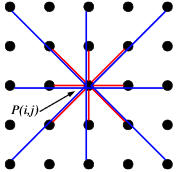
\includegraphics{Figures/choi_ko_model.png}
   \end{center}
   \caption[Choi Ko cloth model]{Choi Ko cloth model \parencite[2]{Choi2002}}
   \label{fig:choi ko model}
\end{figure}
\\This model uses an energy-based approach, of the general formula \ref{eq:general energy equation}\parencite[3]{Bartels2014}, to calculate the forces acting on individual particles.
\begin{equation}
\begin{split}
\label{eq:general energy equation}
  &F = \bigg(\frac{\delta E(S)}{\delta x}, \frac{\delta E(S)}{\delta y}, \frac{\delta E(S)}{\delta z}\bigg)
  \\\text{where:}
  \\&\text{E(S) is an energy function of S, a representation of the cloth's state}
\end{split}
\end{equation}
Two types of interactions are defined, type 1 and type 2. Type 1 interactions model stretch and shear resistances, the red lines in \ref{fig:choi ko model}, and are represented by a linear spring model. Type 2 interactions model bend forces, the blue lines in \ref{fig:choi ko model}, and helps prevent the so called post-buckling instability problem. The interested reader should see \textcite{Choi2002} for more information on the energy functions for each interaction type.

\subsubsection{Justification of Choice}
Mass-spring models are suitable for use in this project as they are efficient and simple to implement; "Mass-spring models are the most efficient as well as the simplest of the cloth models.  This method is one of the most popular techniques for simulating cloth, especially when interactive frame rates are required" \parencite[2]{Zink2007}. As this project is concerned with the real time animation of cloth, mass-spring models are therefore the obvious choice.
\\Mass-spring models are also the most common method of modelling cloth in video games, used in games such as Alan Wake, \parencite[2]{Enqvist2010}, and Hitman: Codename 47, \parencite[1]{Jakobsen2005}, as well as commercial physics engines for games, such as Havok\textsuperscript{\textregistered} and PhysX\textsuperscript{\textregistered}. Again, since this project is concerned with the simulation of cloth for use in a video game, mass-spring models are the logical choice.
\\In particular, the Provot model will be used for this project as the force-based approach requires the solving of a much simpler series of equations than the energy-based approach of the Choi Ko model, and is therefore likely to be more computationally efficient.
\\\\One disadvantage of the mass-spring model is that it does not achieve realistic animation of cloth as "mass-spring systems do not model any specific material and are not related to measured properties of real clothes" \parencite[3]{Wacker2005a}. However, by careful tuning of the spring stiffness coefficients pleasing results can be achieved; \textcite{Mongus2012} have shown that, with tuning, mass-spring models can reproduce the drape of a cloth with an accuracy of 97\%.
\\Another disadvantage of mass-spring models is what Provot calls 'super-elasticity'; springs are allowed to deform too much, leading to unrealistic looking cloth. This is caused because "the springs are “ideal” and they have unlimited linear deformation rate" \parencite[3]{Vassilev2001}. To counter this effect, Provot suggests enforcing length constraints on structural and shear springs. First the position of the particles are updated, then the deformation of the springs are calculated. If this deformation value is greater than some threshold, $\tau_{c}$, then the position of the connected particles are adjusted so the deformation rate equals $\tau_{c}$. Fig \ref{fig:super-elasticity} shows the super-elasticity problem and the results of employing Provot's corrective method. As can be seen, correcting the super-elasticity results in a much more realistic model.

\begin{figure}
\centering
\subfigure[Super-elasticity effect]{\label{fig:super-elasticity}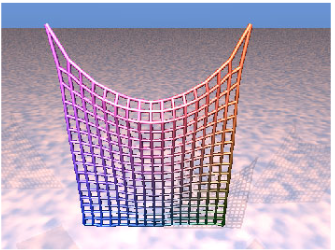
\includegraphics[width=60mm]{Figures/super_elasticity.png}}
\subfigure[Result of correcting super-elasticity]{\label{fig:super-elasticity correction}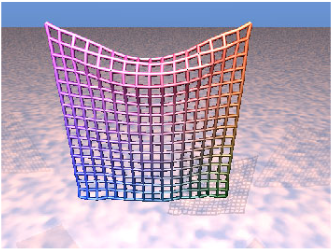
\includegraphics[width=60mm]{Figures/super_elasticity_corrected.png}}
\caption[Super-elasticity problems]{Super-elasticity problems \parencite[4,6]{Provot2001}}
\label{fig:super-elasticity}
\end{figure}

\subsection{Numerical Integration for Mass-Spring Models}
As mentioned above, physically-based models for cloth simulation require solving a series of differential equations, discretised in space and time. According to \textcite[5]{Wacker2005a}, "since particle systems already represent a discretization in space, only a system of ordinary differential equations has to be solved". For the Mass-Spring model using Newtonian mechanics a series of second order ODEs, of the form \ref{eq:newtonian ODE}, must be solved \parencite[5]{Zink2007}.
\begin{equation}
\label{eq:newtonian ODE}
  \frac{\delta^{2}x}{\delta t^{2}} = M^{-1}F(x, v)
\end{equation}
This can be converted into a coupled series of first order ODEs with the addition of an extra variable \parencite[5]{Zink2007}:
\begin{equation}
\label{eq:1st order ODE}
  \frac{\delta}{\delta t} \bigg(\begin{array}{c}  x \\ v \end{array}\bigg) = \bigg(\begin{array}{c}  v \\ M^{-1}F(x, v) \end{array}\bigg)
\end{equation}
Equations \ref{eq:newtonian ODE} and \ref{eq:1st order ODE} cannot be solved analytically, and therefore it is necessary to use a numerical method, or integrator, to approximate them at discrete time intervals. There are many integration methods that could be chosen, typically classified as either explicit or implicit, and the most popular choices will be described now.

\subsubsection{Explicit Integrators}
Most of the early work on physically-based cloth simulation used explicit integrators as they are simple and easy to implement; they only require information about the state of the system at the previous interval to calculate the current state.
\\The most commonly used explicit integrators are the Runge-Kutta family of integrators.

\paragraph{Euler}\leavevmode\\
The first order Runge-Kutta integrator, or explicit Euler, was used in \textcite{Provot2001} to approximate a Mass-Spring system.
\\Equation \ref{eq:1st order ODE} is approximated by \parencite[3]{Wang2009a}:
\begin{equation}
\begin{split}
\label{eq:explicit euler formal}
  &v_{i + \Delta t} = v_{i} + \Delta t F(t_{i}, v_{i})
  \\\text{where:}
  \\&\text{$v_{i}$ and $x_{i}$ are the velocity and position of a particle at time interval i}
  \\&\text{$\Delta t$ is the time step}
\end{split}
\end{equation}
When applied to the Provot Mass-Spring model, this gives \parencite[3]{Provot2001}:
\begin{equation}
\begin{split}
\label{eq:explicit euler provot}
  &a_{i, j}(t + \Delta t) = \frac{1}{m_{i, j}}F_{i, j}(t)
  \\&v_{i, j}(t + \Delta t) = v_{i, j}(t) + \Delta ta_{i, j}(t + \Delta t)
  \\&x_{i, j}(t + \Delta t) = x_{i, j}(t) + \Delta tv_{i, j}(t + \Delta t)
  \\\text{where:}
  \\&\text{$a_{i, j}$, $m_{i, j}$, $v_{i, j}$ and $x_{i, j}$ are the acceleration, mass, velocity and position of particle i, j respectively}
\end{split}
\end{equation}
The explicit Euler method is computationally cheap but can result in numerical instability if too large a time step is used. Mathematically, the explicit Euler method is stable only if the time step is less than the natural period of the system, approximated as $\pi\sqrt{\frac{m}{K}}$, where K is the maximum stiffness in the system. \textcite[2]{Vassilev2001} found that in fact explicit Euler is only stable for $\Delta t$ values less than $0.4\pi\sqrt{\frac{m}{K}}$. 
\\As cloth generally does not stretch easily, this results in high stiffness in the structural and shear springs, which necessitates the use of a small time step if the explicit Euler integrator is chosen. This can impact the overall performance of the simulation, as while this integrator is cheap, the frequency of calculations is high as a result of the time step limitations.

\paragraph{Midpoint}\leavevmode\\
The explicit Midpoint integrator is a second order Runge-Kutta method and modifies the Euler integrator to give greater stability.
\\Equation \ref{eq:explicit euler formal} is modified to give the following \parencite[3]{Wang2009a}:
\begin{equation}
\label{eq:midpoint}
  v_{i + \Delta t} = v_{i} + \Delta t F\bigg(t_{i} + \frac{\Delta t}{2}, v_{i} + \frac{\Delta t}{2}F(t_{i}, v_{i})\bigg)
\end{equation}
Since this method requires two derivatives, the computational cost is greater than Euler. However, because the midpoint method affords greater numerical stability (see fig \ref{fig:stability regions}), a larger time step can be used which increases the overall simulation performance; \textcite{Wang2009a} have shown that the midpoint integrator offers close to twice the simulation performance over explicit Euler.
\begin{figure}[tp]
   \begin{center}
     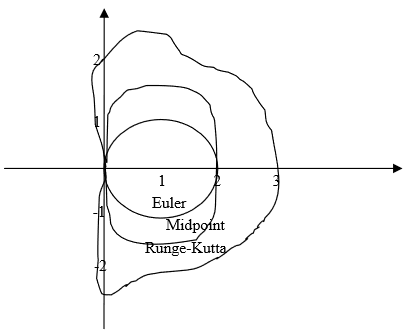
\includegraphics{Figures/stability_diagram.png}
   \end{center}
   \caption[Explicit integrator stability regions]{Explicit integrator stability regions \parencite[4]{Wang2009a}}
   \label{fig:stability regions}
\end{figure}

\paragraph{Fourth order Runge-Kutta}\leavevmode\\
The Fourth order Runge-Kutta integrator offers greater stability using larger time steps over the midpoint method and is formulated as \parencite[3]{Wang2009a}:
\begin{equation}
\begin{split}
\label{eq:4th order rk}
  &v_{i + \Delta t} = v_{i} + \frac{\Delta t}{6}(k_{1} + 2k_{2} + 2k_{3} +  k_{4})
  \\&k_{1} = F(t_{i} + v_{i})
  \\&k_{2} = F\bigg(t_{i} + \frac{\Delta t}{2}, v_{i} + \frac{\Delta t}{2}k_{1}\bigg)
  \\&k_{3} = F\bigg(t_{i} + \frac{\Delta t}{2}, v_{i} + \frac{\Delta t}{2}k_{2}\bigg)
  \\&k_{4} = F\bigg(t_{i} + \Delta t, v_{i} + \frac{\Delta t}{2}k_{3}\bigg)
\end{split}
\end{equation}
This integrator has a significantly higher computational cost than the other methods discussed, however \textcite[4]{Volino2001} have shown that the Runge-Kutta integrator supports time steps almost six times larger than the midpoint method. Therefore, given that Runge-Kutta is three times as computationally expensive as midpoint, this suggests that this integrator can lead to twice the overall simulation performance. \textcite[4]{Wang2009a} have also shown that the fourth order Runge-Kutta integrator offers simulation performance over midpoint and explicit Euler.

\paragraph{Verlet}\leavevmode\\
Verlet integration is an alternative to the Runge-Kutta family of integrators. It avoids velocity calculations by approximating the velocity of a particle using its previous positions.
\\A particle's new position is approximated by \parencite[2]{Mongus2012}:
\begin{equation}
\label{eq:verlet}
  x_{i + \Delta t} = 2x_{i} - x_{i - \Delta t} + a_{i + \Delta t}\Delta t^{2}
\end{equation}
This method is computationally fast and reasonably stable, as "velocity is implicitly given and consequently it is harder for velocity and position to come out of sync" \parencite[1]{Jakobsen2005}. However it does still suffer from time step issues; figures 11 and 13 in \textcite[14-15]{Wacker2005a} show that below a certain threshold Verlet integration is less stable than explicit Euler, but more stable over that threshold.

\subsubsection{Implicit Integrators}

\subsubsection{Position Based Dynamics}

\section{Optimisation}
In simple terms, mathematical optimisation, also known as mathematical programming, is the process of finding the optimal solution to some function based on a set of constraints.
\\Optimisation problems typically take the form\cite{mathprog}:
\begin{equation}
  \begin{split}
    &\text{maximise (minimise) } f(x) : x \text{ in X}
    \\\text{subject to:}
    \\&X \in \mathbb{R}
    \\&g(x) < 0
    \\&h(x) = 0
    \\\text{where:}
    \\&\text{X is the set of values for } x \text{; the domain of the function}
    \\&f(x) \text{ is the function being optimisied; the objective function}
    \\&g(x) \text{, } h(x) \text{ are constraints on } x 
    \\&\text{The number of contraints depends on the optimisation problem}
  \end{split}
\label{eq:optimisation}
\end{equation}
The goal of optimisation techniques is to "find the peak of the fitness landscape"\cite{stoch}. The fitness landscape, or search space, of a function is a plot of the solutions to the function against their fitness value. Each solution is a feasible solution to the function and the fitness of a solution is a measure of its quality, i.e. the result of the objective function. See fig \ref{fig:fitness landscape}\cite{fitland} for an example fitness landscape for the 2D sphere function.
\begin{figure}[tp]
   \begin{center}
     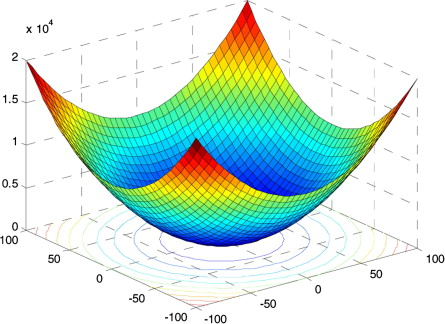
\includegraphics{Figures/sphere_function}
   \end{center}
   \caption{Fitness landscape for the 2D sphere function}
   \label{fig:fitness landscape}
\end{figure}
\\For this project, one type of optimisation technique was studied; stochastic optimisation. 

\subsection{Stochastic Optimisation}
Stochastic optimisation algorithms make use of randomness in order to move through the fitness landscape of the function. This gives this class of algorithm an advantage over more traditional optimisation techniques when dealing with real world problems.
\\Traditional optimisation techniques, such as gradient descent, are deterministic and guarantee to find the optimum solution when dealing with relatively simple problems. However, they are often computationally infeasible on many real world problems or may be unable to optimise the function at all if many local optima are present in the fitness landscape (see fig \ref{fig:local optima}\cite{localo} for an example fitness landscape with local optima).
\begin{figure}[tp]
   \begin{center}
     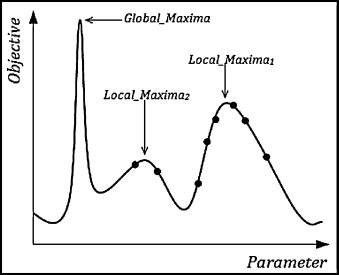
\includegraphics{Figures/local_optima}
   \end{center}
   \caption{A simple fitness landscape showing 2 local optima}
   \label{fig:local optima}
\end{figure}
\\The random aspect of stochastic optimisation means that these algorithms only sample a portion of the solution space which makes them much more computationally feasible on large continuous problems. The randomness also means that stochastic algorithms are capable of "jumping" around the solution space, which allow them to deal with the problem of local optima.
\\A wide variety of stochastic algorithms are available and due to the author's interests, those chosen for this project are computational intelligence techniques.

\section{Computational Intelligence}
Computational Intelligence (CI) is often used in general to refer to artificial intelligence (AI) techniques, but is actually a distinct branch of AI. AI is defined by John McCarthy, considered to have coined the term in 1955, as "the science and engineering of making intelligent machines"\cite{mccarthy}. It is more commonly defined as "the study of the design of intelligent agents"\cite{poole}.
\\CI techniques are designed to replicate observable intelligence mechanism in nature, for example simulating the ways in which the human brain works or the collective intelligence of an ant colony. 
\\This project looked at two CI techniques:
\begin{itemize}
  \item{Evolutionary Algorithms}
  \item{Swarm Intelligence}
\end{itemize}
Both of these techniques are population based, this means they use a population of solutions which are then manipulated to move through the fitness landscape of the function.

\section{Evolutionary Algorithms}
\label{sec:ea}
Evolutionary Algorithms (EAs) are a set of algorithms designed around the principles of natural evolution and Darwinian selection. Carlos A. Coello Coello describes the general structure of an EA as "a population of encoded solutions (individuals) manipulated by a set of operators and evaluated by some fitness function.”\cite{coello}

\subsection{Encoding}
\label{sec:encoding}
Solutions, or individuals, in EAs and other population based algorithms are encoded. This involves mapping the "features" of a solution, i.e. the parameters of the objective function, into a machine readable format. The "features" of a solution are also known as decision variables. This machine readable form is called the \emph{genotype}, and is analogous in nature to DNA. As with DNA, the genotype is expressed (decoded) to give the features, or \emph{phenotype}, of the individual. An individual's genotype is made up of a number of \emph{chromosomes} and each chromosome consists of a number of \emph{genes}. As with nature, the individual genes are responsible for encoding some feature in the phenotype. With EAs, each gene typically encodes one phenotype feature, however it is also possible for one gene to encode multiple features, \emph{pleiotropism}, or for a single feature to be encoded by multiple genes, \emph{polygeny}.
\\The two most common methods of encoding are:
\begin{itemize}
  \item{Binary coding. Each chromosome is represented by a string of binary bits}
  \item{Real value coding. Each chromosome is represented by a string of real values, i.e. the actual phenotype values}
\end{itemize}
Other encoding methods include graph/tree encoding.

\subsection{Operators}
Genetic operators are the methods by which individuals in EAs are moved through the fitness landscape. They are designed to imitate natural processes and introduce \emph{variance} into the population.
\\Three operators are used in EAs, and each algorithm provides their own implementation:
\begin{itemize}
  \item{Selection/Reinsertion. Used to select individuals from the population. Often imitates Darwinian selection; those individuals that are most fit are more likely to survive}
  \item{Recombination. Used to produce new individuals from a number of parent individuals; imitates breeding}
  \item{Mutation. Used to provide further variance in the genotype of individuals; imitates genetic mutation}
\end{itemize}

\subsection{Generic Evolutionary Algorithm}
The structure of EAs is typically the same, first an initial (parent) population is generated. This population is evaluated using the fitness function, and if stopping criteria are met the algorithm exits. If the criteria are not met, then a number of offspring individuals are generated, using selection, recombination and mutation operators. These offspring individuals are evaluated with the fitness function and the reinsertion operator combines the parent and offspring individuals into the population. The stopping criteria are checked again, and if they are still not met this process repeats. See fig \ref{fig:EA} for a diagram\cite{eadiag}, and related pseudocode\cite{eapseudo}, of this process.
\\As mentioned, the stopping criteria are used to end the EA. The simplest and most common form is a limit on the number of iterations for the algorithm; this is almost always included. Another common stopping criteria is to stop when the result of the fitness function is greater than (or less than, depending on maximisation or minimisation) some defined constant. 
\begin{figure}[tp]
   \begin{center}
      \subfigure[Generic EA diagram]{
         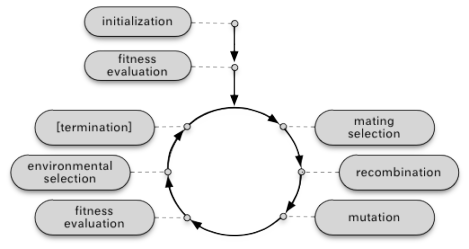
\includegraphics{Figures/ea_diagram}
         }
      \subfigure[Psuedocode for generic EAs]{
         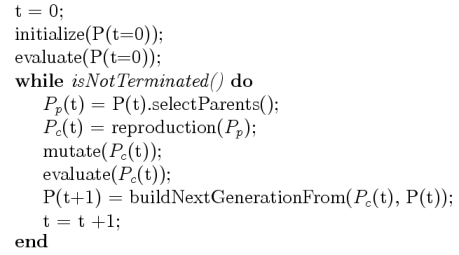
\includegraphics{Figures/ea_pseudo}
         }
   \end{center}
   \caption{Diagram and pseudocode for the operation of a generic EA}
   \label{fig:EA}
\end{figure}

\subsection{Specific Evolutionary Algorithms}
While the section above discussed the generic operation of EAs, this section will detail the specific EA algorithms investigated for this project.
\\There are three main EA variants:
\begin{itemize}
  \item{Genetic Algorithms}
  \item{Evolution Strategies}
  \item{Genetic Programming}
\end{itemize}
The genetic and evolution strategies algorithms were studied for this project, and will now be discussed.

\subsection{Genetic Algorithms}
Genetic Algorithms (GAs) are some of the earliest examples of EAs. First suggested in the late 1950s and early 1960s, these initial algorithms attracted little follow up. It was not until 1975 that interest in GAs took off, with John Holland's book \emph{Adaptation in Natural and Artificial Systems}\cite{4-ga, gahist, pga1}
\\GAs are designed to model genetic evolution and use the selection and recombination operators as the main evolutionary force\cite{4-ga}.

\subsubsection{Encoding}
The canonical GA, as defined by John Holland, use binary coding to encode the individuals in the population; most GA variants use this encoding method (see section \ref{sec:encoding}).
\\The use of binary coding allows the recombination and mutation operators to be very simple but makes the evaluation of an individual's fitness slightly more complex. Before evaluation can be performed, the individual's genotype must be converted (decoded) into its phenotype. An individual I, with n$_{x}$ features will be encoded as: I = (b$_{1}$, ..., b$_{n_{x}}$), where b$_{j}$ is a gene represented as a bit vector of length n$_{d}$. The total number of bits in the bitstring (n$_{b}$) is: n$_{b}$ = n$_{x}$n$_{d}$. b$_{j}$ can be decoded to give f$_{j}$ using the following\cite{4-en}
\begin{equation}
\label{eq:decode}
  f_{j} = x_{min, j} + \frac{x_{max, j} - x_{min, j}}{2^{n_{d}} - 1}(\sum_{l=1}^{n_{d}-1}{b_{j(n_{d}-l)}2^{l}})
\end{equation}
x$_{min}$ and x$_{max}$ are the lower and upper bounds of the search space, meaning that all decoded values will lie in the range [x$_{min}$, x$_{max}$]. As such, GAs are inherently constrained and do not need constraint handling mechanisms (discussed in a later section) to prevent exploration outside the search space.
\\By rearranging equation \ref{eq:decode}, the equation for encoding individuals is obtained:
\begin{equation}
  b_{j} = round(\frac{f_{j} - x_{min, j}}{\frac{x_{max, j} - x_{min, j}}{2^{n_{d}} - 1}})
\end{equation}
\\A slight variation on binary encoding is grey coding. The problem with traditional binary coding is that it introduces \emph{Hamming cliffs}. "A Hamming cliff is formed when two numerically adjacent values have bit representations that are far apart"\cite{4-en}. For example, the number 7 in 4-bit binary is 0111 and the number 8 is 1000. In order to move from 7 to 8, the values of all 4 bits have to change; there is a \emph{Hamming distance} of 4. This can cause problems for a GA, as a larger number of mutations are required to get to 8. Grey coding resolves this problem by ensuring that the Hamming distance between successive numbers is always 1, see table \ref{tab:greycode}.
\begin{table}[tp]
   \begin{minipage}{\textwidth}
      \begin{center}
         \begin{tabular}{c|c|c}
           Value & Binary Code & Grey Code \\
           \hline
           0   & 0000 & 0000 \\
           1   & 0001 & 0001 \\
           2   & 0010 & 0011 \\
	3   & 0011 & 0010 \\
	4   & 0100 & 0110 \\
	5   & 0101 & 0111 \\
	6   & 0110 & 0101 \\
	7   & 0111 & 0100 \\
	8   & 1000 & 1100 \\
	9   & 1001 & 1101 \\
	10 & 1010 & 1111 \\
	11 & 1011 & 1110 \\
	12 & 1100 & 1010 \\
	13 & 1101 & 1011 \\
	14 & 1110 & 1001 \\
	15 & 1111 & 1000
         \end{tabular}
      \end{center}
   \end{minipage}
   \caption{Differences between binary and grey coding}
   \label{tab:greycode}
\end{table}
Binary code is converted into grey code as follows\cite{4-en}:
\begin{equation}
  \begin{split}
    &g_{1} = b_{1} \\
    &g_{l} = b_{l-1}\mathaccent"7016{b}_{l} + \mathaccent"7016{b}_{l-1}b_{l}
  \end{split}
\end{equation}
where b$_{l}$ is the l$^{th}$ bit in the binary code, b$_{1}$ is the most significant bit, \={b}$_{l}$ means not b$_{l}$, + means logical OR and multiplication means logical AND. Grey code values are converted into the phenotype using a modified version of equation \ref{eq:decode}\cite{4-en}
\begin{equation}
  f_{j} = x_{min, j} + \frac{x_{max, j} - x_{min, j}}{2^{n_{d}} - 1}(\sum_{l=1}^{n_{d}-1}{(\sum_{q=1}^{n_{d}-l}{b_{(j-1)n_{d}+q}}})\;mod\;2)2^{l}
\end{equation}
\\Real value encoded GAs have also been proposed. The use of real values makes recombination and mutation more complicated, whilst making evaluation simpler. For this project, only binary or grey coded GAs were considered.

\subsubsection{Selection}
\label{sec:gaselec}
Selection operators in GAs are used for two purposes, first to select individuals for use in recombination (mate selection) and second to select the population of the next generation (reinsertion or environmental selection). There are many selection methods and the canonical GA makes use of proportional selection.
\\\\Proportional selection uses a probability distribution which is sampled to select individuals from the population. This selection method is biased towards the most fit individuals in the population but is not an elitist selection method. Elitist selection methods guarantee that the most fit individual(s) in a population will be selected. With proportional selection, whilst the most fit individuals have a higher probability of selection, it is possible that they may not be selected. The probability of selection for each individual is calculated using its fitness value\cite{4-se, eoselect, gaselect, gatsp}
\begin{equation}
  P(x_{i}) = \frac{f(x_{i})}{\sum_{j=1}^{n}{f(x_{j})}}
\end{equation}
Once the probability of selection for each individual has been calculated and combined into a probability distribution, you can sample it and select as many individuals as necessary.
\\Proportional selection is also known as roulette wheel selection. Sampling the probability distribution can be thought of as spinning a roulette wheel, where each individual has been assigned a portion of the wheel proportional to their selection probability (see fig \ref{fig:roulette}\cite{rw}).
\begin{figure}[tp]
   \begin{center}
     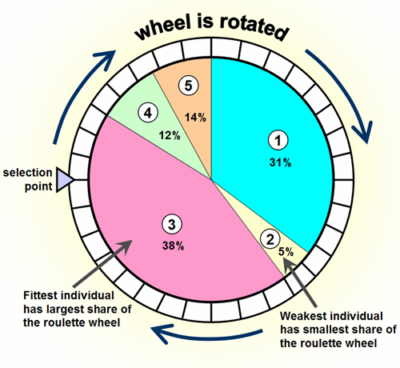
\includegraphics{Figures/roulette_wheel}
   \end{center}
   \caption{Representation of roulette wheel selection}
   \label{fig:roulette}
\end{figure} 
\\Proportional selection as defined here will not work for minimisation problems, as the most fit individuals will be assigned a small probability of selection. In order to use proportional selection for minimisation problems, the fitness values of the population need to be scaled. One method of scaling is\cite{4-se}
\begin{equation}
  scaled fitness(x_{i}) = f_{max} - f(x_{i})
\end{equation}
with f$_{max}$ as the maximum possible fitness value. If the maximum possible fitness is not known, then the maximum observed fitness, f$_{max}$(t), can be used. Another scaling method is\cite{4-se}
\begin{equation}
  scaled fitness(x_{i}) = \frac{1}{1 + f(x_{i}) - f_{min}(t)}
\end{equation}
The advantage of proportional selection is that it preserves diversity by affording all individuals a probability of selection\cite{gatsp, eoselect}. However, due to the direct relationship between the fitness of the individuals and the selection probabilities, it is possible for a small number of very fit individuals to dominate selection, potentially resulting in premature convergence\cite{4-se, gatsp}.
\\\\Rank based selection is another selection method. This is similar to proportional selection, except that instead of using the fitness values to directly calculate selection probabilities, the fitness values are used to assign the individuals a rank. The population is first sorted according to the fitness values, and then the individuals are assigned a rank, either so the best individual has rank n (where n is the population size)\cite{gaselect} or rank 0\cite{4-se}. The rank of the individual is then used to calculate the selection probability. The resulting probability distribution can then be sampled to select individuals. Methods to assign selection probabilities include the linear ranking method
\begin{equation}
  \begin{split}
  &P(x_{i}) = \frac{1}{N}(\eta^{-}+(\eta^{+}-\eta^{-})\frac{i-1}{N-1})\text{\cite{gaselect}} \\
  &or \\
  &P(x_{i}) = \frac{1}{N}(\eta_{max}-2(\eta_{max}-1)\frac{i-1}{N-1}\text{\cite{eoselect}}
  \end{split}
\end{equation}  
For this project however, the following method is used\cite{l2}:
\begin{equation}
\label{eq:rank}
  P(x_{i}) = \frac{rank(x_{i})}{\sum_{j=1}^{n}{rank(x_{j})}}
\end{equation} 
This method was chosen due to its simplicity and the previous experience of the author.
\\Rank based selection attempts to deal with the disadvantage of proportional selection; that a few very fit individuals are able to dominate the selection. Because the fitness values are not used directly in calculating the selection probability this problem is avoided. It does not matter how much more fit the best individual is compared with the others, it will only be one rank higher. Rank based selection has its own disadvantages though, it can be computationally expensive, due to the need to sort the population, and may still lead to premature convergence as the best chromosomes are not so strongly differentiated\cite{gatsp}.
\\\\A third selection method is tournament selection. This is a commonly used method due to its simplicity and efficiency. A number of individuals are randomly selected from the population, and the best individual is selected\cite{4-se, eoselect, gaselect, gatsp}. The number of individuals selected from the population each time is called the tournament size. Careful selection of the tournament size is important in order to prevent the best or worst individuals from dominating, leading to a reduction in diversity\cite{4-se, gatsp}. A common tournament size is 2, and tournaments of this variety are called \emph{binary tournaments}\cite{gaselect, gatsp}.
\\For details on other selection methods, see \cite{4-se} and \cite{gaselect}.

\subsubsection{Recombination}
The recombination operator for GAs is called crossover. When dealing with binary or grey coded GAs, crossover generally involves swapping sections of the bitstrings between two parent individuals. This is an example of \emph{sexual} crossover, where two parents individuals are used to produce one or two offspring.\emph{ Asexual}; one parent producing one offspring, and \emph{multi-recombination}; more than two parents producing one or more offspring, crossover variants also exist but for this project only sexual methods were investigated.
\\A bit mask, the same length as the bitstring, is used to control which bits are exchanged between the parent individuals. The bit mask is read a bit at a time, and if the bit is set, the corresponding bits in the parents are exchanged to produce offspring (see algorithm \ref{alg:crossover}\cite{4-ga}).
\begin{algorithm}[tp]
\label{alg:crossover}
  \SetAlgoLined
  offspring1 = parent1, offspring2 = parent2\;
  Compute bit mask m\;
  \For{i = 1, ..., n}{
    \If{m[i] = 1}{
      offspring1[i] = parent2[i]\;
      offspring2[i] = parent1[i]\;
    }
  }
\caption{Using a bit mask for crossover}
\end{algorithm}
The purpose of a crossover operator is to compute the bit mask. Three operators have been developed for binary crossover, fig \ref{fig:operators_a}\cite{gacross} shows a summary of the three.
\begin{itemize}
  \item{One-point crossover. One point in the bitstring is randomly selected, this is called the crossover point. The bit mask is computed such that all bits after the crossover point are set. Used by the canonical GA}
  \item{Two-point crossover. Two points in the bitstring are randomly selected; a start and end point. The bit mask is computed such that all bits between these two points are set. Fig \ref{fig:operators_b}\cite{l2} shows an example of two-point crossover with the bit mask}
  \item{Uniform crossover. A random bit mask is generated. Each bit in the mask has a probability of being set. Fig \ref{fig:operators_c}\cite{l2} shows an example of uniform crossover with the bit mask}
\end{itemize}
\begin{figure}[tp]
   \begin{center}
      \subfigure[Crossover operators]{
         \label{fig:operators_a}
         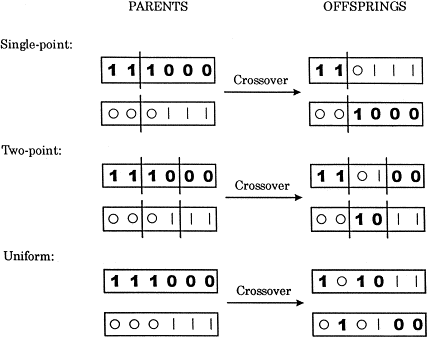
\includegraphics{Figures/crossover}
         }
      \subfigure[Two-point crossover with bit mask]{
         \label{fig:operators_b}
         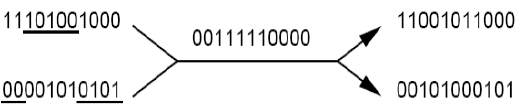
\includegraphics{Figures/2point}
         }
      \subfigure[Uniform crossover with bit mask]{
         \label{fig:operators_c}
         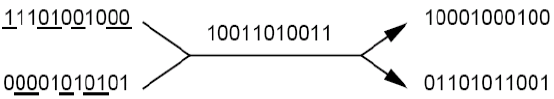
\includegraphics{Figures/uniform}
         }
   \end{center}
   \caption{Summary showing the three sexual crossover operators \subref{fig:operators_a} with bit masks \subref{fig:operators_b}, \subref{fig:operators_c}}
   \label{fig:operators}
\end{figure}
A configurable parameter controls crossover. Called the \emph{crossover rate}, it is effectively the probability that crossover will take place. Generally, a high crossover rate is used; between 0.5 and 1\cite{4-ga, garates}.

\subsubsection{Mutation}
Mutation is applied to the offspring produced by crossover in order to add further genetic variation to the population. In binary or grey coded GAs, the process is very simple; the value of certain bits is inverted. The bits to invert are selected using one of two methods
\begin{itemize}
  \item{Uniform mutation. Bits are chosen at random and inverted. Used by the canonical GA}
  \item{Inorder mutation. Similar to two-point crossover, a start and end point is randomly selected and all bits between these points are inverted.}
\end{itemize}
Gaussian mutation similar to that used in ES (see section \ref{sec:es_mutation}) can be used for GAs where the phenotype is floating-point numbers. The genotype is first decoded into the phenotype, gaussian mutation is applied and then the result is converted back into the genotype.\cite{4-ga}
\\As with crossover, mutation is controlled by a parameter, called \emph{mutation rate}. This is the probability with which the selected bits are inverted. Typically a small value is used for the mutation rate\cite{4-ga, garates}.

\subsubsection{Configurable Parameters}
A GA has a number of configurable parameters that can affect the performance and output of the algorithm. Careful selection of these parameters is essential to optimise the performance of the GA, and while they may be problem dependent and number of standards have been established\cite{gap, iga}.
\\The key parameters are
\begin{itemize}
  \item{Population size}
  \item{Number of generations}
  \item{Number of bits to represent each gene}
  \item{Selection method and tournament size (if appropriate)}
  \item{Crossover type and rate. Crossover is explorative, meaning it is used to discover good search areas; \emph{exploring} the search space. So the crossover rate needs to be high to allow the algorithm to find the global optimum}
  \item{Mutation type and rate. Mutation is exploitative, meaning it explores locally within an area. So the mutation rate should be small in order to reduce the size of the area searched and prevent good solutions being changed too much. If the mutation rate is too small however, very little exploration will take place and the population may converge to a local optimum}
\end{itemize}

\subsection{Evolution Strategies}
First developed in the 1960s by Rechenberg and later by Schwefel, Evolution Strategies (ES) are based on the idea of "the evolution of evolution"\cite{4-es}. Unlike GAs which are designed to replicate evolution on a genetic level, ES are designed on species-level evolution; the emphasis is towards the phenotype rather than the genotype.
\\The first ES suggested was the (1 + 1)-ES and does not use a population; one individual is used and one offspring is produced using a mutation operator\cite{4-es, es}. The first multimembered ES, ($\mu$ + 1), was developed by Rechenberg. It uses $\mu$ parents, selects 2 randomly and produces one offspring from them and the best $\mu$ individuals are selected into the population\cite{4-es, es}. Schwefel later introduced two more multimembered ES: ($\mu$, $\lambda$) and ($\mu$ + $\lambda$)\cite{es}, which use a population of $\mu$ parents and produce $\lambda$ offspring. These types of ES are often shown as $(\mu\;\overset{+}{,}\;\lambda)$.

\subsubsection{Encoding}
ES individuals are encoded using real value coding, which better reflects the focus on the phenotype of the individuals. There is therefore no need to decode the individuals before fitness evaluation, as the values of the decision variables are stored directly.
\\In addition to the set of decision variables, individuals in ES are also coded with a set of strategy parameters. The strategy parameters are used to control the mutation operator and influence the search direction and step size\cite{4-es, es}. The use of strategy parameters means that an ES always moves towards the optimum which give ES an advantage over GAs, which can move in any direction. As such, it is expected that ES have a faster convergence speed than GAs.
\\It is incredibly important to adjust the value of the strategy parameters throughout the evolution process, otherwise the ES loses it's evolvability\cite{es}. The traditional way of mutating the strategy parameters was using the 1/5th-rule\cite{es}. However, this restricts the number of strategy parameters to one and is really only applicable to (1 + 1)-ES. A better way to adjust the strategy parameters is \emph{self-adaptation}. Self-adaptation means that the strategy parameters are evolved at the same time as the decision variables; the strategy parameters undergo recombination and are mutated along with the decision variables.

\subsubsection{Selection}
Selection in ES is much simpler than in GAs; the $\mu$ best individuals are selected from a pool of individuals. How the pool of individuals is populated depends on the type of ES. 
\\\\With ($\mu$ + $\lambda$)-ES, the pool of individuals is the combination of the $\mu$ parents and the $\lambda$ offspring. This method places no limits on the number of offspring, since you can always guarantee that at least $\mu$ individuals will be in the selection pool. This is an elitist selection method; it always ensures that the most fit individuals will survive into the next generation\cite{4-es, es, esc}. It is possible with this selection method for parent individuals to survive in the population indefinitely. In order to prevent this, ($\mu$ + $\lambda$) can be enhanced to ($\mu$, $k$, $\lambda$), where $k$ is the lifespan of an individual; individuals will be discarded if they exceed their lifespan\cite{4-es}.
\\\\For ($\mu$, $\lambda$)-ES, the selection pool is the $\lambda$ offspring only, the parent individuals are discarded. Therefore, this selection method requires that $\mu$ < $\lambda$. This selection method is not elitist, as the parents are discarded, and therefore results in greater diversity within the population\cite{4-es, es, esc}.

\subsubsection{Recombination}
As opposed to GA recombination, ES recombination produces only one offspring from $\rho$ parents, where $2 \le \rho \le \mu$. Recombination where $\rho = 2$ is called local recombination and when $\rho > 2$ is called global\cite{4-es}, or multi\cite{es}, recombination. There are two simple methods of recombination, \emph{discrete} and \emph{intermediate}.
\\Discrete recombination is denoted as $(\mu/\rho_{D}\;\overset{+}{,}\;\lambda)$. In this method, each decision variable in the offspring corresponds directly to the decision variable in a randomly selected parent. For a parent decision vector $a$ = ($a_{1}, ..., a_{n}$) and an offspring $r$ = ($r_{1}, ..., r_{n}$),\cite{es}
\begin{equation}
  \begin{split}
    &r_{k} = (a_{p})_{k} \\
    &\text{where } p = random[1, ..., \rho]
  \end{split}
\end{equation} 
So, the $k^{th}$ component of $r$ is the $k^{th}$ component of the $p^{th}$ parental vector, $a$, with $p$ as a random parent.
\\Intermediate recombination is denoted as $(\mu/\rho_{I}\;\overset{+}{,}\;\lambda)$ and uses the average value of the decision variables in the parents to produce the offspring. For a parent decision vector $a$ = ($a_{1}, ..., a_{n}$) and an offspring $r$ = ($r_{1}, ..., r_{n}$),\cite{es}
\begin{equation}
  r_{k} = \frac{1}{\rho}\sum_{p=1}^{\rho}{(a_{p})_{k}}
\end{equation} 
So, the $k^{th}$ component of $r$ is the average value of the $k^{th}$ component in all the parental vectors, $a$.

\subsubsection{Mutation}
\label{sec:es_mutation}
Mutation in ES happens with a probability of 1, as opposed to a very low probability in GAs. Mutation takes place in two steps, first mutation (self-adaptation) of the strategy parameters and then mutation of the decision variables.
\\When there is only one strategy parameter, an offspring $y$ is mutated to $y'$ as follows\cite{4-es, es}
\begin{equation}
  \begin{split}
    &y' = y + z \\
    &\text{where } z = \sigma(N_{1}(0, 1), ..., N_{n}(0, 1))
  \end{split}
\end{equation}
Each decision variable of $y$ is mutated by $\sigma(N(0, 1))$, where $\sigma$ is the strategy parameter and $N(0, 1)$ is a random sample from a Gaussian (normal) distribution; hence why ES mutation is called Gaussian mutation.
\\This can be modified to support multiple strategy parameters\cite{4-es, es}
\begin{equation}
  \begin{split}
    &y' = y + z \\
    &\text{where } z = (\sigma_{1}N_{1}(0, 1), ..., \sigma_{n}N_{n}(0, 1))
  \end{split}
\end{equation}
Now, a separate strategy parameter is used to mutate each decision variable in the offspring. Obviously, this now requires that the number of strategy parameters and decision variables are the same; $n_{s} = n_{d}$.
\\\\The most common method of mutating strategy parameters is the log-normal method, so called because of the logarithmic normal distribution it generates
\\A strategy parameter, $\sigma$, is mutated to $\sigma'$ using the log-normal method as follows\cite{4-es, es}
\begin{equation}
  \begin{split}
    &\sigma' = \sigma exp(\tau N(0, 1)) \\
    \text{where } \\
    &\tau = \frac{1}{\sqrt{n}} \\
    &n \text{ is the size of the search space, i.e. the number of decision variables}
  \end{split}
\end{equation}
This method of mutation works for one strategy parameters, and is slightly modified if more than one strategy parameter needs mutating.
\\A strategy parameter, $\sigma_{i}$, in a set $\sigma = (\sigma_{1}, ... \sigma_{n})$, is mutated to $\sigma'_{i}$ as follows\cite{4-es, es}
\begin{equation}
  \begin{split}
    &\sigma'_{i} = \sigma_{i}exp(\tau'N(0, 1))exp(\tau N_{1}(0, 1)) \\
    \text{where } \\
    &\tau' = \frac{1}{\sqrt{2n}} \\
    &\tau = \frac{1}{\sqrt{2\sqrt{n}}} \\
    &n \text{ is the size of the search space, i.e. the number of decision variables}
  \end{split}
\end{equation}

\subsubsection{Constraint Handling}
\label{sec:constraints}
Unlike GAs, ES are not inherently bound to a finite search space. Unconstrained, an ES will explore outside the bounds of a search space to find the optimum. If the algorithm is required to only search a finite space then a method of constraint handling must be implemented. Constraint handling methods are also implemented to handle any other constraints that there may be on the function being optimised, so the techniques listed here are also applicable to GAs in that sense. Constrained optimisation problems split the search space into feasible and infeasible regions. Figure \ref{fig:feasible}\cite{constraints} shows the feasible and infeasible regions for some function. It might be the case that to reach the optimum the algorithm needs to pass through an infeasible region, so constraint handling mechanisms should still allow infeasible solutions to be selected. For example, in fig \ref{fig:feasible}, if the optimum was at $d$, the algorithm would have to move through the infeasible region to reach it.
\begin{figure}[tp]
   \begin{center}
     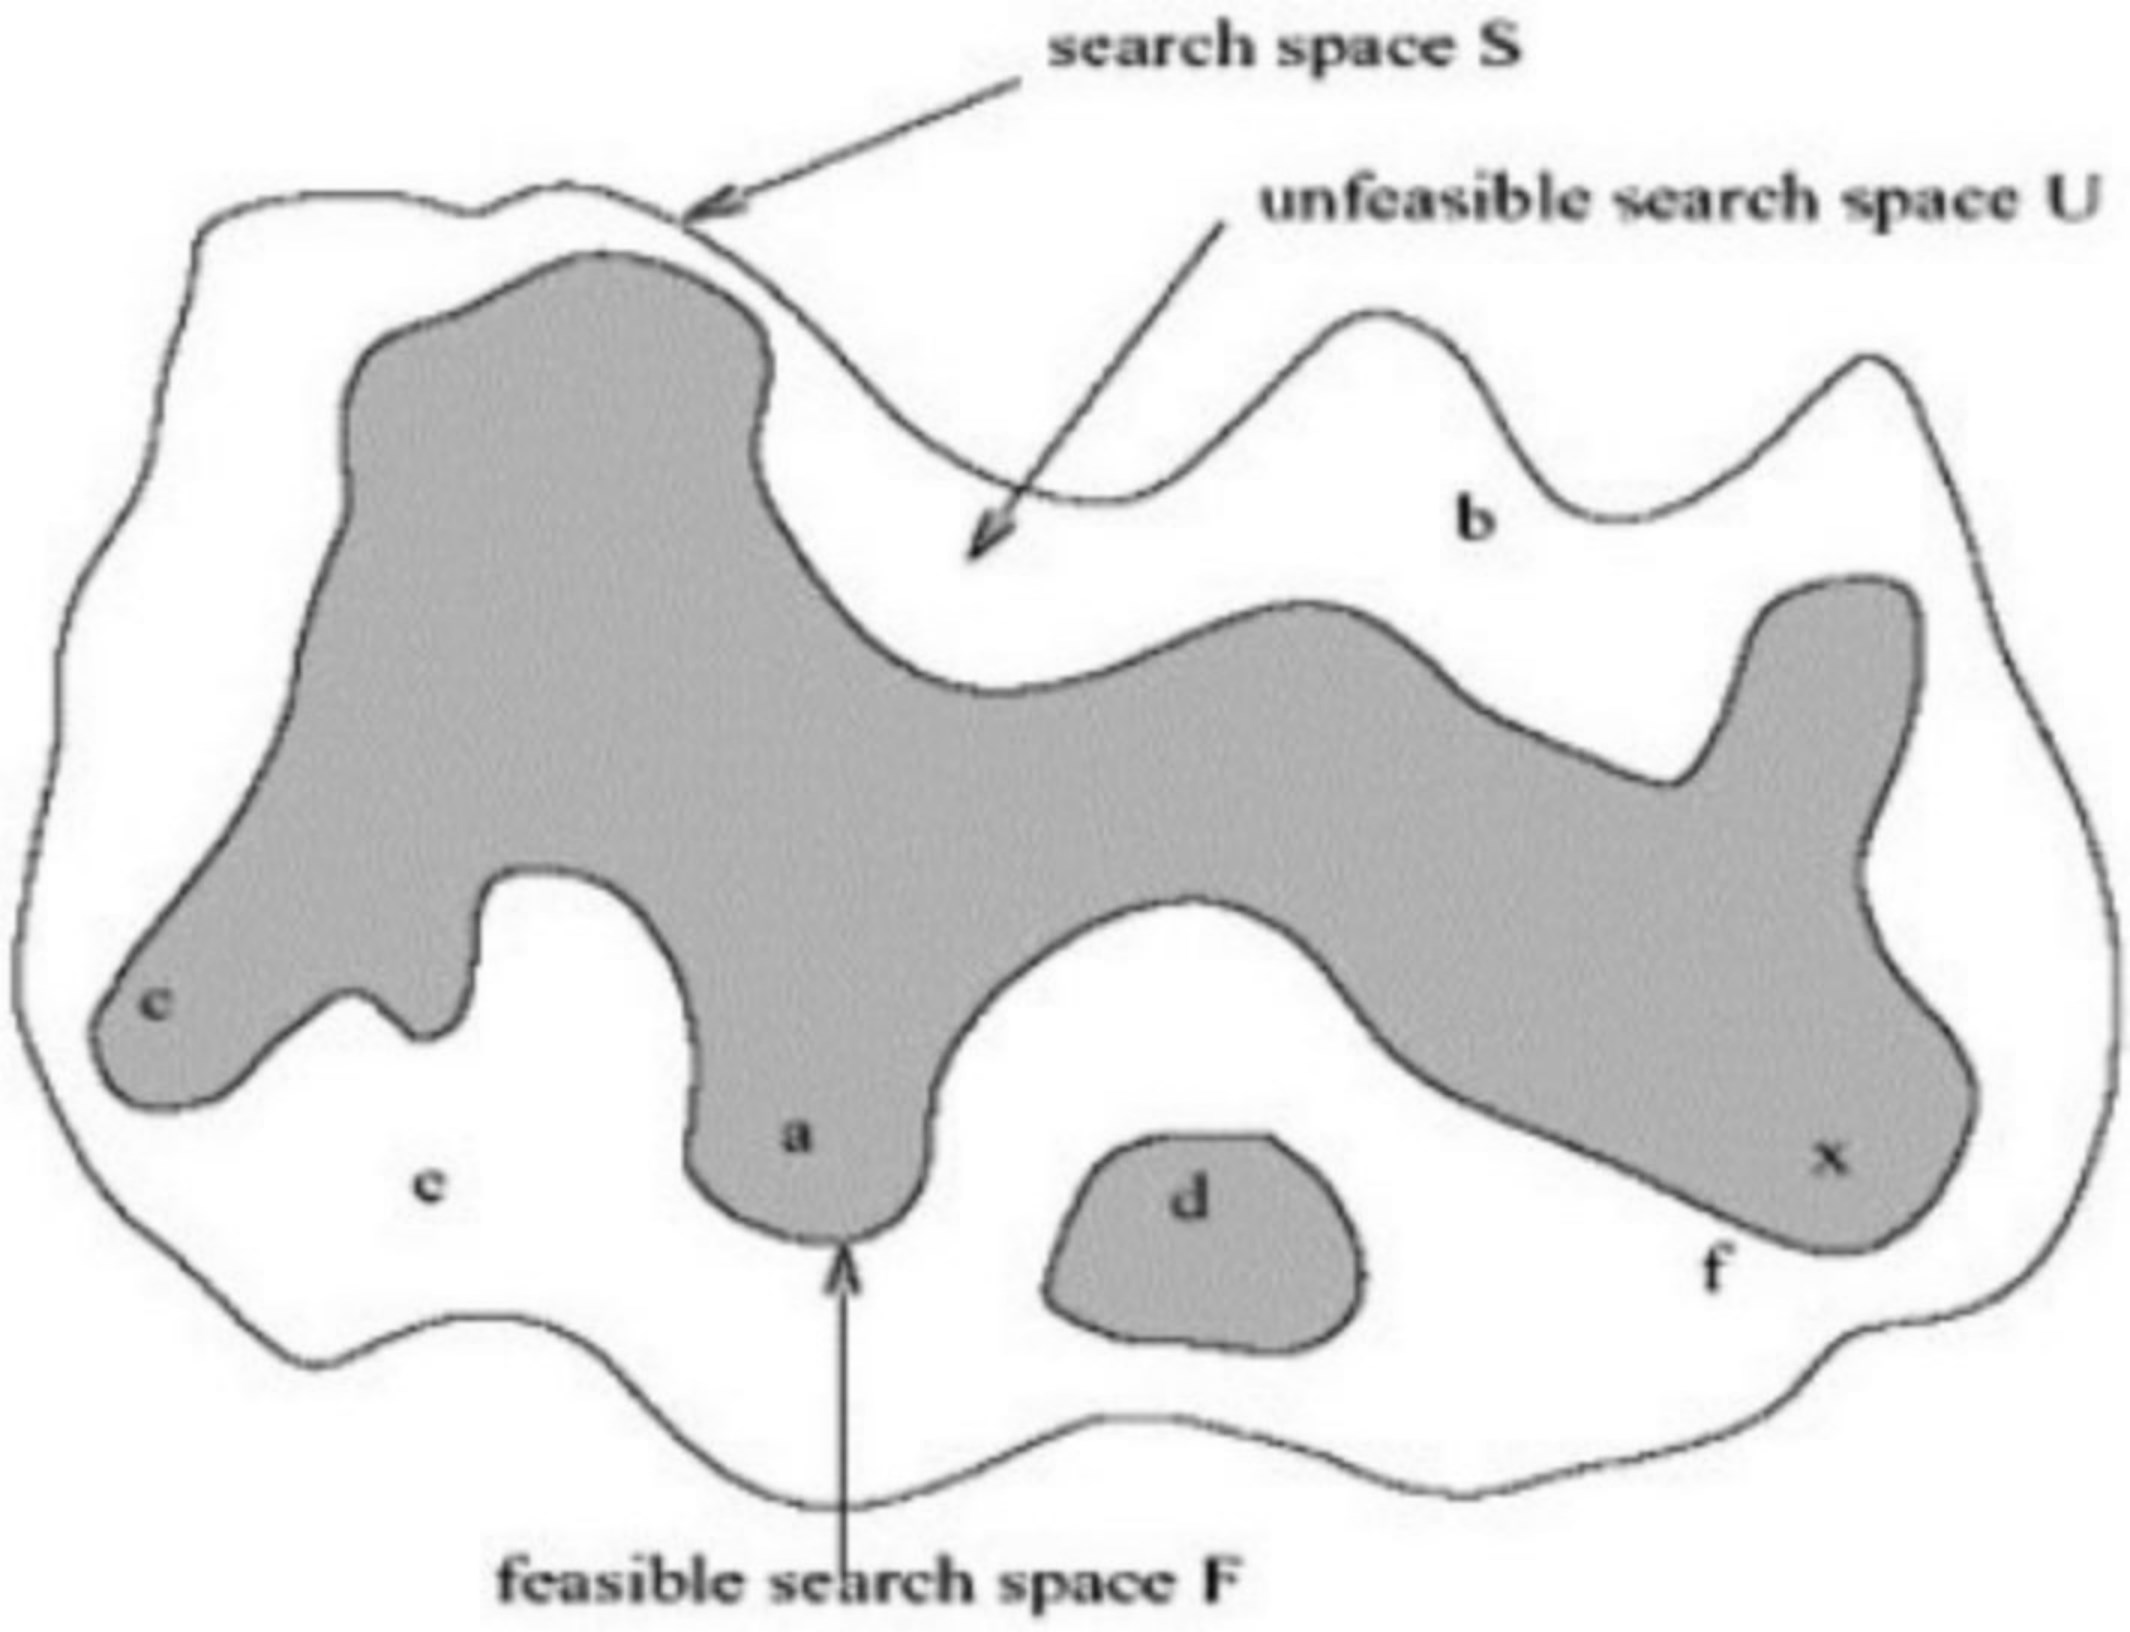
\includegraphics{Figures/feasible}
   \end{center}
   \caption{A search space, showing the feasible and infeasible regions}
   \label{fig:feasible}
\end{figure}
\\\\One method of constraint handling are \emph{penalty functions}. With penalty functions, the constrained problem is converted into an unconstrained problem by adding a term to the fitness function which is "based on the amount of constraint violation"\cite{gecco}. For a constrained optimisation problem defined as in equation \ref{eq:optimisation}, a penalised fitness function is usually takes this form\cite{4-ga, gecco}
\begin{equation}
  \begin{split}
    &f'(x) = f(x) \pm (\sum_{i=1}^{n}{r_{i}G_{i}} + \sum_{j=1}^{p}{c_{j}L_{j}}) \\
    \text{where} \\
    &G_{i}\text{ is a function of the constraints }g(x)\text{, typically }max[0, g_{i}(x)]^{\beta} \\
    &L_{j}\text{ is a function of the constraints }h(x)\text{, typically }|h_{j}(x)|^{\gamma} \\
    &\beta\text{ and }\gamma\text{ are usually 1 or 2} \\
    &\text{Equality constraints }h(x) = 0\text{ are converted to inequality constraints }|h(x)| - \varepsilon \le 0 \\
    &\varepsilon\text{ is the tolerance allowed (small)} \\
    &r_{i}\text{ and }c_{j}\text{ are constants called penalty factors}
  \end{split}
\end{equation}
\\There are various methods for defining the value(s) of the penalty factors.
\\\\Static penalty factors are one approach, and use constant penalty factors. One method, suggested by Homaifar, Lai and QI in 1994, defines multi- levelled penalty factors based on the level of constraint violation. Higher levels of violation have higher penalty factors. The penalised fitness if calculated as follows\cite{4-ga, constraints, gecco}
\begin{equation}
  \begin{split}
    &f'(x) = f(x) + (\sum_{i=1}^{n}{R_{j, i}G_{i}}) \\
    &\text{where }R_{j, i}\text{ is the }j^{th}\text{ violation level for constraint }i
  \end{split}
\end{equation}
This method has some disadvantages, primarily that a large number of parameters need to be created; each constraint has a number of violation levels that need to be created and penalty factors may be problem dependent\cite{constraints, gecco}.
\\\\Dynamic penalty factors are another approach, and involves the generation number in setting the penalty factors. Using this approach, the penalty factors increase over time. Joines and Houck suggest a method where the penalised fitness is calculated by\cite{4-ga, esc, constraints, gecco}
 \begin{equation}
  \begin{split}
    &f'(x) = f(x) + (C.t)^{\alpha}(\sum_{i=1}^{n}{G_{i}^{\beta}(x)}) \\
    &\text{where }C\text{, }\alpha\text{, }\beta\text{ are user defined constants and }t\text{ is the generation number} \\
    &\text{typically }C = 0.5\text{, }\alpha = 1\text{ or } 2\text{ and }\beta = 1\text{ or } 2
  \end{split}
\end{equation}
Experiments have shown that the values of C, $\alpha$ and $\beta$ can seriously affect the performance of an EA, potentially leading to premature convergence or convergence to a local optimum\cite{constraints}
\\\\Another method of constraint handling is to simply reject infeasible individuals. This is often called the \emph{death penalty} method. This approach is very simple, infeasible solutions are discarded and new solutions generated until there are enough feasible solutions. This method works reasonably well with large feasible search spaces but has been shown, by experiment, to perform badly with small feasible regions\cite{esc, constraints, gecco}.
\\\\Repair methods are a third constraint handling mechanism. These methods make use of a repair algorithm which "generates a feasible solution from an infeasible one"\cite{esrev}. The repaired solution can then be used to evaluate its infeasible equivalent, or it can replace the infeasible solution in the population\cite{constraints, esrev}. The specifics of the repair algorithm are usually problem dependent, so there are few standard repair techniques\cite{constraints}.
\\Many other constraint handling mechanisms exist, see \cite{constraints} for details.

\subsubsection{Configurable Parameters}
ES have similar configuration parameters to GAs.
\\The key parameters are
\begin{itemize}
  \item{Population size}
  \item{Number of generations}
  \item{Number of strategy parameters}
  \item{Selection method}
  \item{Number of offspring to produce. Must be greater than $\mu$ if using $(\mu,\lambda)$ selection}
  \item{Number of parents to use to produce offspring}
  \item{Recombination method}
\end{itemize}

\section{Swarm Intelligence}
A \emph{swarm} can be defined as "a group of (generally mobile) agents that communicate with each other (either directly or indirectly), by acting on their local environment"\cite{4-IV}. Swarm intelligence is the complex behaviour and problem-solving abilities developed by a swarm. Individuals in a swarm are simple, so the complex behaviour swarms exhibit come from the interactions between individuals, as opposed to the individuals themselves. This is called \emph{emergence}\cite{4-IV}. Swarms of bees, ant colonies and bird flocks are natural examples of intelligent swarms and swarm intelligence algorithms aim to simulate this.
\\Whilst many swarm intelligence algorithms exist, this report is concerned with only one, Particle Swarm Optimisation (PSO).

\subsection{Particle Swarm Optimisation}
Developed in the 1990s by James Kennedy and Russell Eberhart, PSO attempts to model the behaviour of birds in a flock\cite{4-pso, mopso}. The complex behaviour displayed by PSO is that of "all individuals converging on the environment state that is best for all individuals"\cite{4-IV}, i.e. the global optimum. It can be thought that individuals, or particles, in the population are 'flown' around the solution space "according to its own experience and that of its neighbours"\cite{4-pso, mopso}.

\subsubsection{Basic Particle Swarm Optimisation Algorithm}
PSO is much simpler than EAs, discussed in section \ref{sec:ea}. There are no complex encoding methods or genetic operators. Particles are represented as a position (the decision variables) and velocity vector and each iteration the position and velocity of each particle is updated. The position of particle $i$ at time $t$, $x_{i}(t)$, is updated using the velocity of the particle, $v_{i}(t)$\cite{4-pso, mopso, psot}
\begin{equation}
  x_{i}(t+1) = x_{i}(t) + v_{i}(t+1)
\label{eq:pos}
\end{equation}
The velocity of the particles reflects both the experience of the particle (\emph{cognitive component}) and the experience of neighbouring particles (\emph{social component}). The size of the particle's neighbourhood can vary, and this gives rise to different PSO variants. The original two variants are \emph{gbest} and \emph{lbest}.

\subsubsection{gbest Particle Swarm Optimisation}
In a gbest, or \emph{global best}, PSO, a particle's neighbourhood is the entire swarm. This means the social component of each particle's velocity is taken from all the particles. In this case, the social component is the best value found by any particle in the swarm (\emph{global best value}). Hence, the velocity for a particle is updated as follows\cite{4-pso, psot} \begin{equation}
  \begin{split}
    &v_{i}(t+1) = v_{i}(t) + c_{1}r_{1}(pbest_{i}(t) - x_{i}(t)) + c_{2}r_{2}(gbest(t) - x_{i}(t)) \\
    \text{where } \\
    &c_{1}\text{ and }c_{2} \text{ are user supplied acceleration constants, typically set to 2\cite{psot, psoi}} \\
    &r_{1}\text{ and }r_{2}\text{ are fresh uniform random numbers} \\
    &pbest_{i}(t)\text{ is the \emph{personal best value}, i.e. the best value seen, of individual }i
  \end{split}
\label{eq:gvel}
\end{equation}
This gives us the pseudocode for a gbest PSO, see algorithm \ref{alg:gbest}.
\begin{algorithm}[tp]
\label{alg:gbest}
  \SetAlgoLined
  initialise a population; \\
  \While{stopping criteria not met}{
    update global best value; \\
    \For{all particles}{
      update personal best value; \\
      update velocity vector using equation \ref{eq:gvel}; \\
      update position vector using equation \ref{eq:pos}; \\
    }
  }
\caption{gbest Particle Swarm Optimisation algorithm}
\end{algorithm}

\subsubsection{lbest PSO}
A lbest, or \emph{local best}, PSO, uses a neighbourhood of the $k$ nearest neighbours of a particle. The social component of a particle's velocity is still the best value found by the neighbourhood, but a small neighbourhood is used now; the social component is called the \emph{local best value}. The velocity for a particle is updated by\cite{4-pso}
 \begin{equation}
  \begin{split}
    &v_{i}(t+1) = v_{i}(t) + c_{1}r_{1}(pbest_{i}(t) - x_{i}(t)) + c_{2}r_{2}(lbest_{i}(t) - x_{i}(t)) \\
    \text{where } \\
    &c_{1}\text{ and }c_{2} \text{ are user supplied acceleration constants, typically set to 2\cite{psot, psoi}} \\
    &r_{1}\text{ and }r_{2}\text{ are fresh uniform random numbers} \\
    &pbest_{i}(t)\text{ is the \emph{personal best value}, i.e. the best value seen, of individual }i \\
    &lbest_{i}(t)\text{ is the local best value of the neighbourhood of individual }i
  \end{split}
\label{eq:lvel}
\end{equation}
This gives us the pseudocode for a lbest PSO, see algorithm \ref{alg:lbest}.
\begin{algorithm}[tp]
\label{alg:lbest}
  \SetAlgoLined
  initialise a population; \\
  \While{stopping criteria not met}{
    \For{all particles}{
      update local and personal best values;
      update velocity vector using equation \ref{eq:lvel}; \\
      update position vector using equation \ref{eq:pos}; \\
    }
  }
\caption{lbest Particle Swarm Optimisation algorithm}
\end{algorithm}

\subsubsection{Inertia Weight}
Another variant on the velocity update equation is to add an inertia weight component. The inertia weight controls the influence the previous velocity has on the new velocity\cite{4-pso, mopso, psoi}. Taking the gbest velocity equation (equation \ref{eq:gvel}), adding an inertia weight changes the equation to the following
 \begin{equation}
  \begin{split}
    &v_{i}(t+1) = \omega v_{i}(t) + c_{1}r_{1}(pbest_{i}(t) - x_{i}(t)) + c_{2}r_{2}(lbest_{i}(t) - x_{i}(t)) \\
    &\text{where }\omega\text{ is the inertia weight component}
  \end{split}
\label{eq:inertia}
\end{equation}
The conventional use of inertia weight components is as a static constant, typically defined between 0.8 and 1.2\cite{psot}. A better way to use inertia weights is as a varying weight.
\\A large inertia weight encourages the PSO to be more explorative and a small inertia weight makes the PSO more exploitative. As such, it makes sense to decrease the value of the inertia weight over time; called a \emph{time-varying inertia weight}. This will allow the particles to widely explore the search space at the start of the algorithm, preventing it getting stuck at local optima, and then explore with greater detail in a local area, ensuring that the global optimum will be found.
\\A time-varying inertia weight is usually linearly decreased at each iteration, from a maximum value, $w_{max}$ to a minimum value, $w_{min}$. $w_{max}$ is usually set to 0.9 and $w_{min}$ to 0.4\cite{4-pso, psoi}. The inertia weight is updated using the following equation\cite{4-pso, psoi, vi}
\begin{equation}
  \begin{split}
    &w(t) = \frac{(w_{max} - w_{min})(t_{max} - t)}{t_{max}} + w_{min} \\
    &\text{where } t_{max}\text{ is the maximum number of iterations} \\
  \end{split}
\end{equation}
\\There are other methods of adjusting the inertia weight, see \cite{4-pso} for details.

\subsubsection{Velocity Clamping}
Velocity clamping is used to prevent velocity explosion; where the velocity of the particles rapidly increases to large values, meaning the positions of the particles are updated in large jumps. Essentially, a PSO with velocity explosion is too explorative; the particles explore outside the bounds of the search space. To prevent this, a new parameter is introduced, $v_{max}$. This sets a maximum limit on velocity of a particle and if the updated velocity exceeds this value, it is set to $v_{max}$\cite{4-pso, psot, psoi}. In an optimisation problem bounded by $[-x_{max}, x_{max}]$, the value of $v_{max}$ is\cite{psot}
\begin{equation}
  \begin{split}
    &v_{max} = kx_{max} \\
    &\text{where } k\text{ is a user defined constant, the \emph{velocity clamping factor}} \\
  \end{split}
\end{equation}
If the problem is not bounded by $[-x_{max}, x_{max}]$, but instead by $[x_{min}, x_{max}]$, then the value of $v_{max}$ is determined by\cite{4-pso, psot}
\begin{equation}
  \begin{split}
    &v_{max} =\frac{k(x_{max} - x_{min})}{2} \\
  \end{split}
\label{eq:vmax}
\end{equation}
The value $k$ has been shown to be problem dependent and should be defined in the range \\(0, 1]\cite{4-pso, psot}.
\\For particles with more than one search dimension, a separate $v_{max}$ should be used for each dimension, using the corresponding $x_{min}$ and $x_{max}$.
\\One problem with velocity clamping is when all the velocities are equal to $v_{max}$. In this case, it may prevent the PSO from finding the optimum. The use of an inertia weight can help to prevent this. Another solution is to dynamically decrease $v_{max}$ over time, starting with a large value to allow exploration; dynamic velocity clamping is not discussed in this report, see \cite{4-pso}.

\subsubsection{Bound Handling}
When dealing with constrained optimisation problems, many of the constraint handling methods used in EAs, see section \ref{sec:constraints}, are appropriate. It is important that the way the personal best and neighbourhood best values are updated handles infeasible solutions too, i.e. the personal or neighbourhood best should only be changed for particles in feasible regions\cite{4-pso}. Several methods have been defined for dealing with variable bounds (called \emph{bound handling}) in PSO, and some of which will be discussed briefly here.
\\\\The simplest bound handling method is the random method. The particle's position vector is checked sequentially, and if a variable exceeds its bounds it is moved to a random location between $x_{min}$ and $x_{max}$. This method can have a great impact on convergence accuracy due its random nature\cite{psobh}.
\\\\The set on boundary method is another simple bound handling method. Using this method, variables that exceed their bounds are set to the value of the bound they exceed, e.g. if $x_{max}$ is exceeded, the variable will be set to $x_{max}$. A variant of this method makes use of \emph{velocity reflection}; if a particle's $i^{th}$ variable is set to the boundary, then the $i^{th}$ velocity will by reflected such that the particle is moving in the opposite direction\cite{psobh}.
\\\\A third bound handling method is exponential distribution. This approach adjusts the position of any infeasible variable to a point between its original position and the bound it exceeded. The position of the variable is sampled from a probability distribution calculated such that positions near the bound have a higher selection probability\cite{psobh}.
\\More details on these bound handling methods and a few others can be found in \cite{psobh}.

\subsubsection{Configurable Parameters}
PSO has very few configurable parameters, and the majority are the same as ES and GAs
\\The key parameters are
\begin{itemize}
  \item{Population size}
  \item{Number of generations}
  \item{Velocity clamping factor, k, if using velocity clamping}
\end{itemize}

\section{Connect 4}
Connect 4 is a 2-player game where each player has the same number of identical counters in different colours; typically red and yellow. The goal of each player is to connect four of their counters in either a vertical, horizontal or diagonal line, the first player to do so is the winner. If all the counters for both players have been played without connecting four in a line, then the game is a draw. The game is played on a grid of varying size, but usually 7 columns by 6 rows, and is gravity based, meaning that when a counter is placed into a column it will fall to the lowest unoccupied row in that column.
\\\\Connect 4 was solved in 1988 by Victor Allis and James D. Allen independently. In his master's thesis, Allis describes 9 strategic rules by which to play Connect 4. These rules are based on controlling the \emph{Zugzwang}, a concept Allis defines as forcing "a player to make a move which he would rather not make"\cite{connect4}. The rules Allis defines are listed below. An explanation of the rules has been left out, due to their the relative complexity; interested readers should see \cite{connect4}.
\begin{itemize}
  \item{Claimeven}
  \item{Baseinverse}
  \item{Vertical}
  \item{Aftereven}
  \item{Lowinverse}
  \item{Highinverse}
  \item{Baseclaim}
  \item{Before}
  \item{Specialbefore}
\end{itemize}
Allis also describes a program, VICTOR, which plays Connect 4 using these rules. Using VICTOR, Allis proved that, given perfect play, the first player will always win if they play the first move in the middle column, will always lose if they play the first move in columns 1 and 7, and will always draw if they play the first move in any other column\cite{connect4}.

\section{Technologies}

\subsection{The Arena}
The Arena is a Java based framework developed to allow player "modules" to play against each other automatically. The Arena provides a number of games that modules can be developed to play, but the primary game is Connect 4. It also provides a number of predefined modules, with which to test new modules. New modules can be created by simply implementing an interface, and providing an implementation of a function which returns the next move to play in the game. This function is called each turn by The Arena, and the move returned is played. Each turn is restricted by a time limit, and the opponent will win automatically if the time limit is exceeded by a player. This allows the effectiveness of modules, such as the recursive module, which analyse the future states of the board to find the best move, to be limited; as only so many states can be analysed in the time limit. The Arena also provides a method of storing a move which will be automatically played if the turn time limit runs out; allowing modules like the recursive module to continue to analyse the board until the very end of their turn. 
\\Once a new module is written it simply needs to be published as a jar file and then it can be loaded into The Arena. 
\\The Arena provides both a command line and graphical user interface (GUI). The GUI provides a graphical representation of the board as well as menus to load player modules and set the turn time limit; it is more suited to a human player playing against the computer. The command line interface is much more powerful. It allows tournaments to be set up, where player modules are played against each other over a number of rounds and allows a machine to be set up as a host for a tournament, allowing the games to be run on multiple slave machines, reporting the results back to the host via TCP.
\\\\Since The Arena is Java based, the main development language for this project was Java.

\subsection{Computational Intelligence Libraries}
There are a number of libraries providing CI algorithms, some of which are listed in table \ref{tab:lib}. However, due to the project's aims and the author's goals, the use of a library was not considered for the main body of this project, and the algorithms chosen where implemented from scratch.
\begin{table}[tp]
   \begin{minipage}{\textwidth}
      \begin{center}
         \begin{tabular}{c|c}
           Library & Supported Algorithms \\
           \hline
           ECJ \cite{ecj}                      & GAs, ES, PSO + more \\
           cilib \cite{cilib}                     & GAs, ES, PSO + more \\
           JGAL \cite{jgal}                   & GAs \\
           JGAP \cite{jgap}                 & GAs \\
  	JSwarm-PSO \cite{jswarm} & PSO
         \end{tabular}
      \end{center}
   \end{minipage}
   \caption{Java computational intelligence libraries}
   \label{tab:lib}
\end{table}
\\However, as part of the last aim of the project, it would be helpful to compare the performance of the produced algorithms against those implemented by a popular CI library. As table \ref{tab:lib} shows, there are a number of appropriate Java libraries. However, due to the author's previous experience and time limitations, the Shark machine learning library\cite{shark} was chosen. Shark release 2.3.4\cite{sharksf} was used as at the time of development, this was the most up to date release build available.
\\As Shark is a C++ based library, and this project was developed in Java, the performance comparisons could not be against run speed, as C++ (a compiled language) has an advantage over Java (an interpreted language). Instead, the convergence speed and accuracy of the algorithms would be compared.